\section{Introduction} \label{sec:intro}


Recently, large language models (LLMs) like GPT-4~\cite{openai2024gpt4} and Llama~\cite{touvron2023llama} have shown impressive performance improvements across a variety of natural language processing (NLP) tasks \cite{LeiWANG186345,MuningWEN176349,DerongXU186357,YufeiZENG176340,wu2024survey,liu2024unimel}. However, when dealing with specialized knowledge not in training corpus and complex knowledge reasoning, LLMs still struggle with outdated knowledge and hallucination problems \cite{ji2023survey}. They thus may produce factually incorrect outputs, limiting their usefulness in the areas requiring high reliability, such as healthcare \cite{he2023survey,liu2024moe} and safety \cite{dong2024attacks}. 
 % which have garnered considerable attention from researchers to explore their capabilities for complex knowledge reasoning \cite{TOG}
To solve complex reasoning with specialized knowledge, a line of research \cite{chatkbqa,TOG} have explored Knowledge Graph Question Answering (KGQA), a task that improves logical reasoning and prediction of answers by retrieving reliable information from large-scale knowledge graphs (KGs) like Freebase~\cite{bollacker2008freebase} and Wikidata~\cite{wikidata}. KGs store extensive factual knowledge in a structured format known as triplets \cite{xu2024multi,xu2022relation,wang2023federated}, consisting of \textit{(head entity, relation, tail entity)}, which is seen as a potential solution for enhancing the interpretability of LLMs reasoning \cite{TOG}.
\begin{figure}[t]
\centering
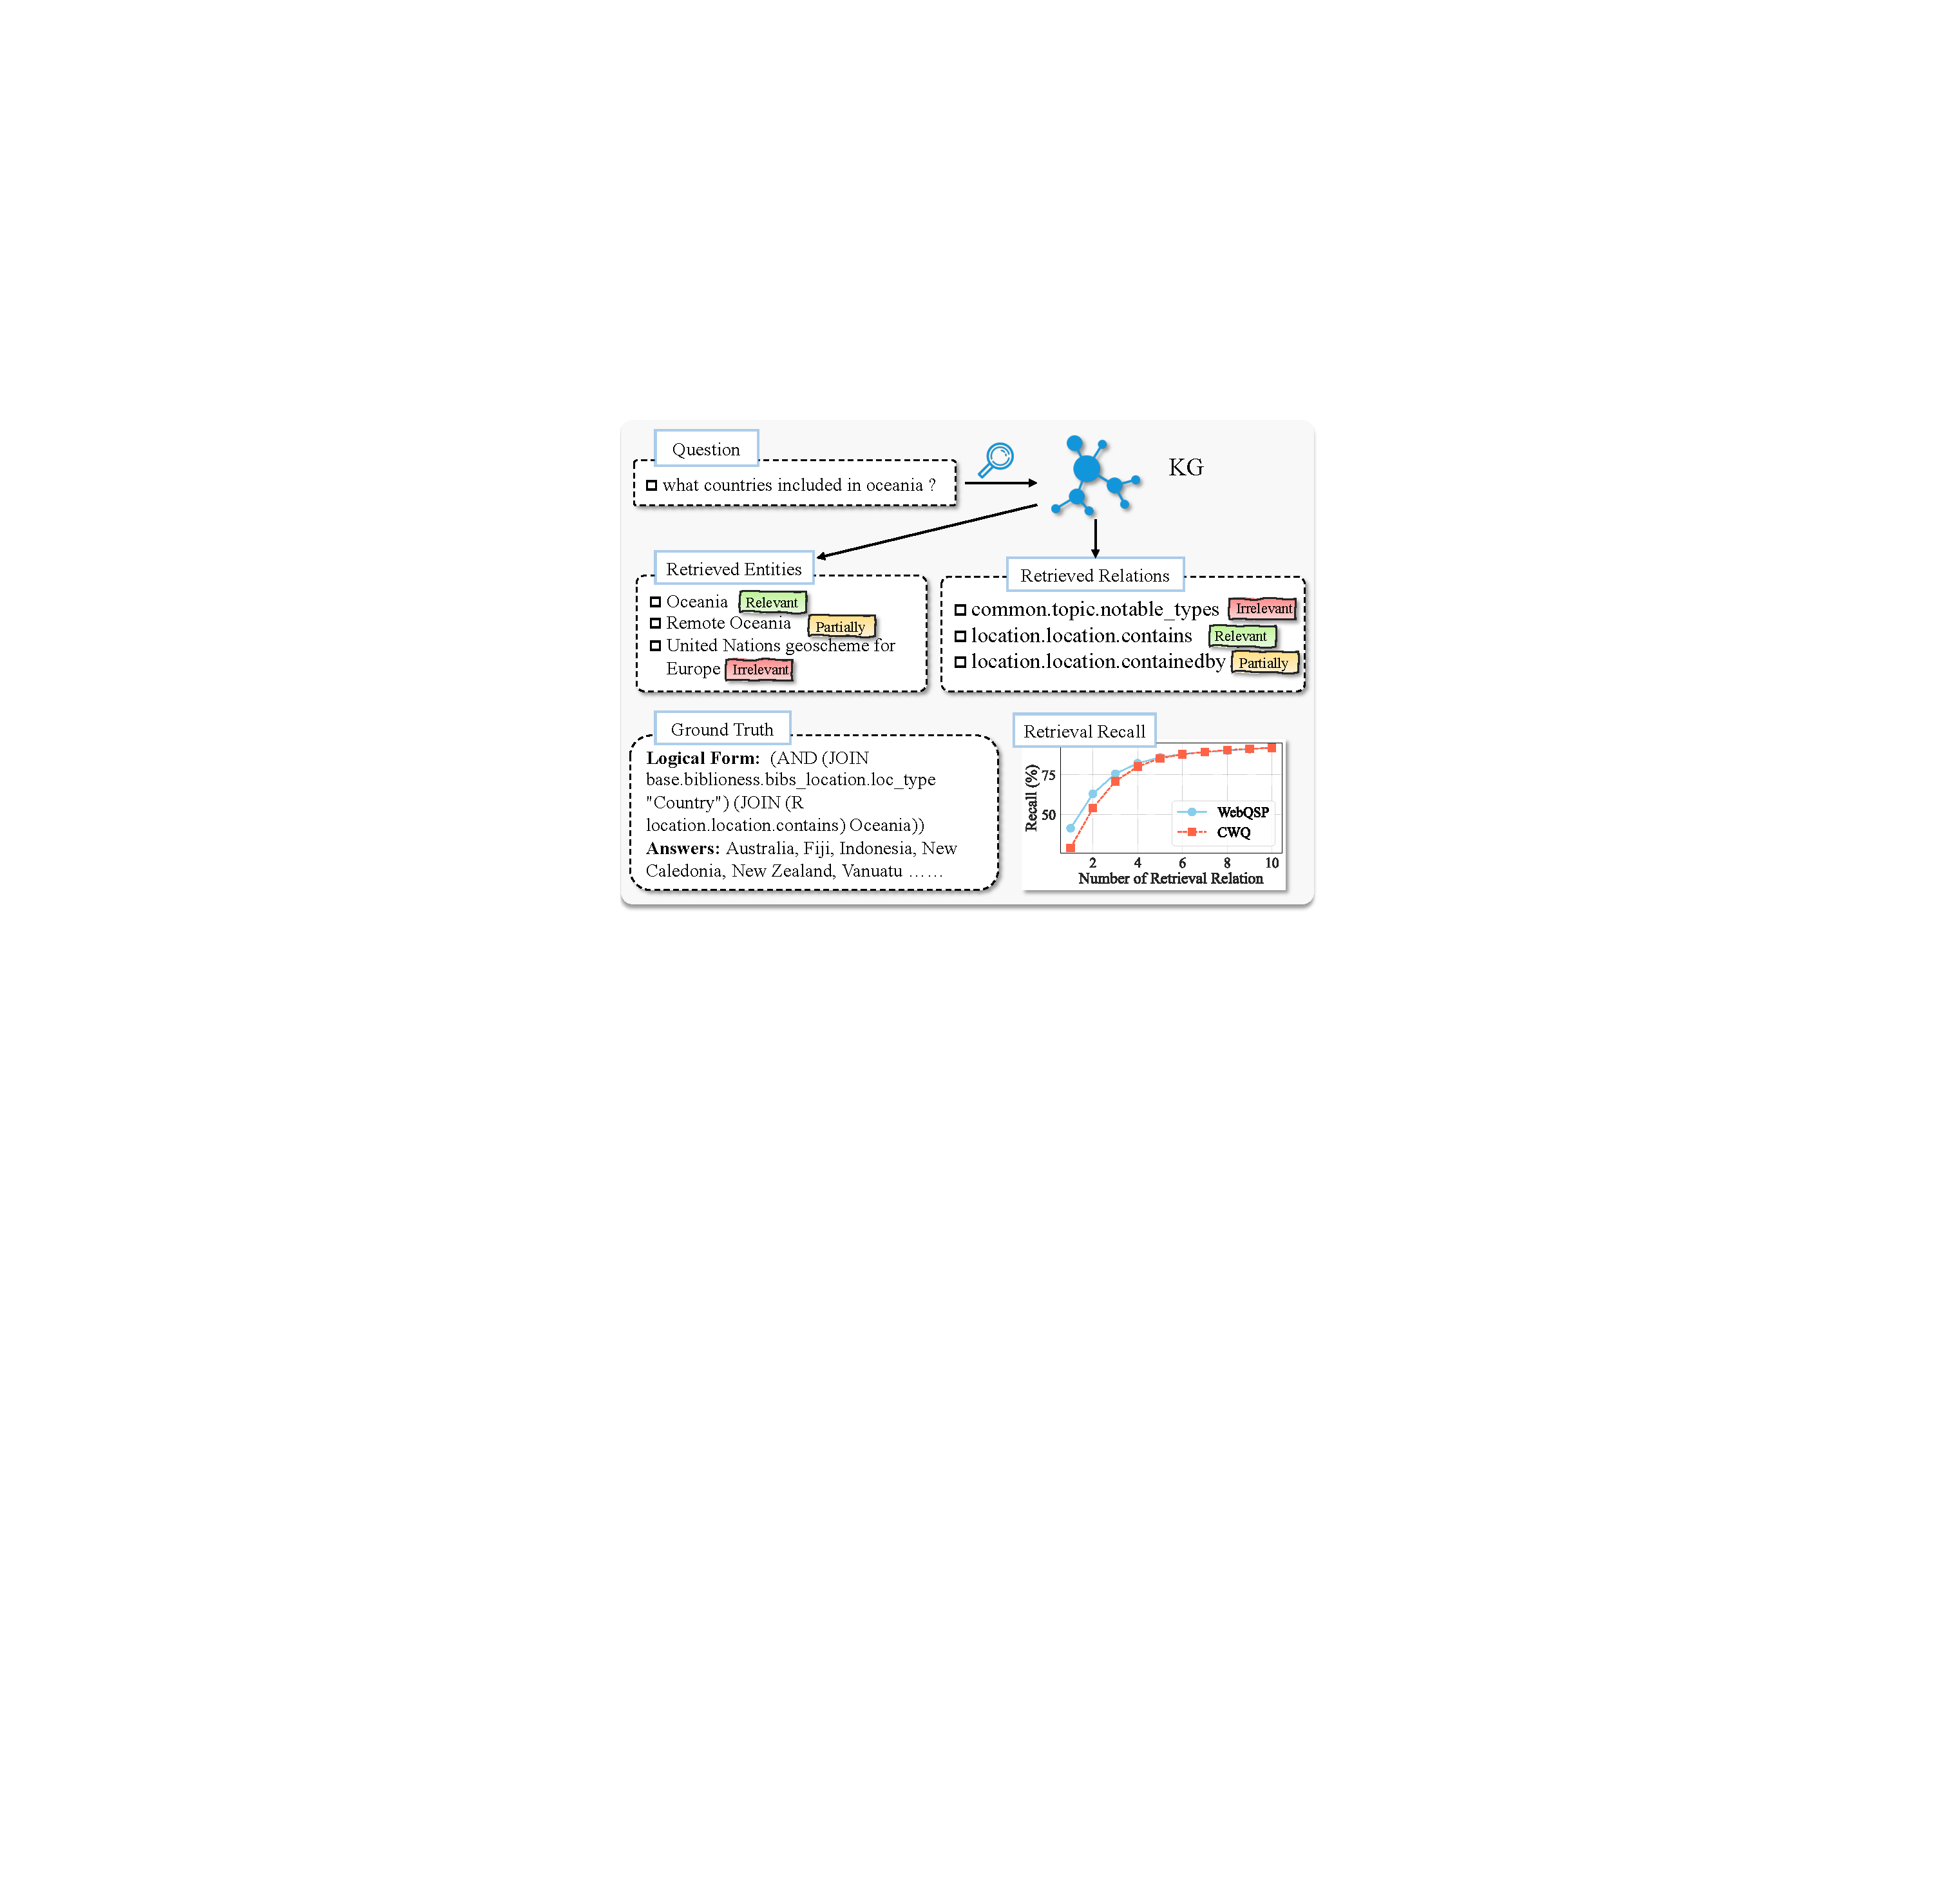
\includegraphics[width=0.9\linewidth]{img/intro.pdf}
\caption{ An example illustrates the retrieval results categorized as \textit{relevant}, \textit{irrelevant}, and \textit{partially relevant}.
}
\label{fig:intro}
\end{figure}

The recent advancements in KGQA can be broadly classified into two main categories.
The first category involves using LLMs to transform input questions into structured logical forms~\cite{chatkbqa}, such as S-expressions, which can then be queried on KG using a graph database query language like SPARQL to obtain the final answers. These approaches leverage the structured nature of KG to extract precise information in response to complex queries.
The second category of KGQA involves directly predicting answers using LLMs without extra logical forms. Some works in this category perform multi-hop reasoning on KG in a step-by-step manner by querying LLMs \cite{TOG}. Other works retrieve additional contextual information related to the question and use it as contextual input to enhance LLMs~\cite{G-retriever,RoG}. These approaches aim to improve the accuracy of answers by incorporating more context into the reasoning process.
% 

However, the retrieval process often yields a large amount of information, as shown in Figure~\ref{fig:intro}, which may be irrelevant or only partially relevant to the question and ground truth. The retrieval recall curve demonstrates a positive correlation between the number of retrieved data and the recall score, indicating that the retrieved data contain valuable information.
Therefore, it raises a question: \textit{How to identify which retrieved knowledge is valuable and which is not?} This question becomes particularly crucial when a significant portion of retrieved knowledge does not provide substantial assistance. In terms of this, we observed that previous studies \cite{decaf,GMT-KBQA} failed to considering commonalities among different aspects of retrieved information, which can be beneficial in identifying crucial knowledge. And they also neglected adaptive learning to establish relevance between question and retrieved text.
 
To address these overlooked challenges, we propose an \underline{a}daptive \underline{m}ulti-\underline{a}spect \underline{r}etrieval-augmented over KG (\textsc{Amar}) framework. Instead of directly appending the retrieved information as context input, \model utilizes the retrieved information more flexibly, therefore enhancing LLMs reasoning.
\model primarily includes two modules:
 1) Self-alignment module, where multi-aspect retrieval data (including entities, relations, and subgraphs, all of which are linearized as text) is separately mapped into prompt embeddings from text, facilitating fine-grained tuning. Next, cross-attention and self-attention are applied to the multi-aspect embeddings to obtain consistency tokens. The aim is to align the commonalities among different pieces of information. For instance, if an entity and a subgraph both mention ``\textit{Oceania}'', this implies that they are probably consistent in conveying the same piece of information. In this way, we can enhance crucial knowledge, thereby reducing noise interference.
 2) Relevance gating module, which measures the relevance between the embedding of question and consistency tokens. This module introduces siamese networks with shared weights to learn relevance score, which serves as a soft gate to adaptively decide which retrieved information is more useful for LLMs reasoning.
Through the self-alignment and relevance gating modules, \model adaptively filters and selects multi-aspect retrieval knowledge, enabling a more rational utilization of context and avoiding interference from noise. We then fine-tune LLM in a parameter-efficient manner to leverage the retrieved knowledge, assisting in generating reasonable logical forms. Finally, we refine the logical forms using the similarity of entities and relations and query KG to obtain final answers.
Overall, this work makes three key contributions:
\begin{itemize}%[topsep=0pt, partopsep=0pt, leftmargin=13pt, parsep=0pt, itemsep=3pt]
    \item To the best of our knowledge, this is the first study to enhance LLMs reasoning for KGQA tasks by utilizing multi-aspect KG information as prompt embeddings. 
    \item  We propose novel self-alignment and relevance gating modules, which enable LLMs to adaptively filter and select multi-aspect retrieval knowledge, allowing for more rational utilization of context while effectively avoiding interference from noise.
    \item The effectiveness of \model was extensively validated on two datasets across five metrics. \model demonstrated superior performance, achieving state-of-the-art (SOTA) results compared to 22 strong baselines.
\end{itemize}

